% !TEX root = master.tex


\chapter{The BGK Model}
\label{CH: BGK}
%\pagenumbering{arabic}




This section covers the kinetic gas model, the BGK model, on which a model order reduction will be performed in the following. In addition the SOD-shocktube, on which the BGK model will be tested is discussed.\\
\section{Discretization, conservative properties and equilibirum}
The BGK model was introduced by, and named after, physicists Prabhu L. Bhatnagar, Eugene P. Gross and Max Krook in 1954 \cite{BGK}. It is an approximation of the standard Boltzmann transport equation. More precisely the r.h.s of the Boltzmann equation is approximated by the BGK operator \cite{puppo2019kinetic}
\begin{equation}
\partial_t f + v \partial_x f = \frac{1}{\tau} (M_f - f) \text{.}
\label{Eq:BGK}
\end{equation}
It consists of the relaxation time \(\tau(x,t)\), the Maxwellian distribution \(M_f\) and \(f(x,v,t)\) the probability of a gas particle having a microscopic velocity \(v\) in phase space \((x,v,t)\). The left side of the BGK model is a transport equation for \(f(x,v,t)\) with transport velocity \(v\). In the maxwellian distribution \(n(x,t)\) is the number of particles in space and time, \(R\) is the specific gas constant, \(T^0(x,t)\) is the temperature and \(u(x,t)\) is the macroscopic velocity
\begin{equation}
M_f = \frac{n(x,t)}{\sqrt{2\pi R T^0(x,t)}}\exp(-\frac{(v - u(x,t))^2}{2 R T^0(x,t)}) \text{.}
\end{equation}
Note that in this thesis the BGK model is discussed in one dimension. Hence the BGK model needs to be evaluated for three independent variables \(x\), \(v\) and \(t\) as seen above.\\ 
Now what makes the BGK model especially attractive for model order reduction?
The fruitfullness of performing a model order reduction on the BGK model becomes clearer when looking at it's space and velocity discretization
\begin{equation}
	\partial_t f_{j,k} = -(v_k)_1D_x f|_{j,k}(t) + \frac{1}{\tau}({M_f}_{j,k}(t) - f_{j,k}(t)) \text{.}
	\label{Eq:Discrete BGK}
\end{equation}
Here a uniform grid is considered with \(x_j = j\Delta x\), \(j \in \mathbb{Z}\), \(v_k = k\Delta v\), \(k \in \mathbb{Z}\) and \(t^n = n \Delta t\), \(n \in \mathbb{N}\) on which \(f_{j,k} = f(x_j,v_K,t)\) and \({M_f}_{j,k} = M_f(x_j,v_k,t)\) are evaluated at point \((x_j,v_k)\) in a time instance \(t\). For brevity \(D_x f|_{j,k}\) is the discrete space derivative at \((x_j,v_k)\) \cite{puppo2019kinetic}. Now the PDE in \cref{Eq:BGK} is broken down into a system of ODE's in time, for which every ODE is a lineaar advection equation with constant scalar speed \(v_k\) and a source term.\\ 
To continue let's consider \(K\) to be the number of gridpoints in velocity and \(J\) to be the number of grid points in space. Then a total of \(KJ\) first order differential equations need to be evaluated in 1D. Obviously in three dimensions the system of ODE's inflates up to \(K^3N^3\) first order differential equations \cref{Eq:Discrete BGK}. This in turn drives the evaluation of the BGK model at the edge of intractability for dense meshes in 3D and all together stimulate the want for a reduced order model.\\
\begin{wrapfigure}{r}{0.5\textwidth}
	\vspace{-10pt}
	\begin{center}
		\scalebox{.9}{% This file was created by tikzplotlib v0.9.6.
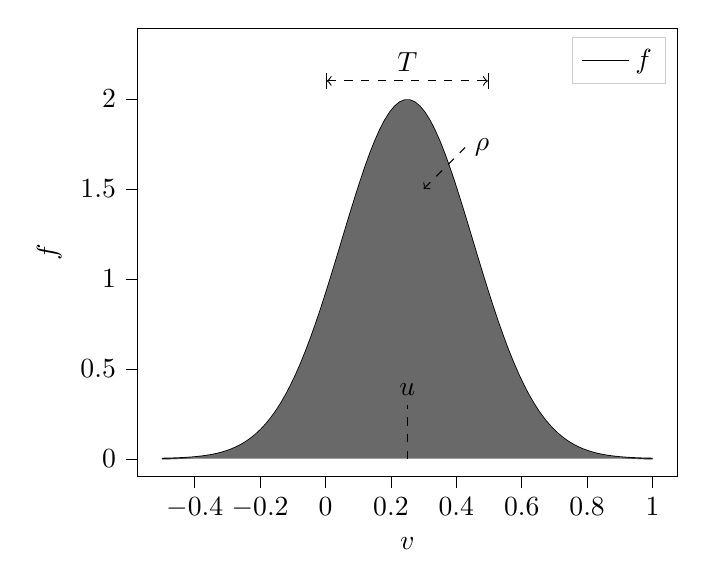
\begin{tikzpicture}

\begin{axis}[
legend cell align={left},
legend style={fill opacity=0.8, draw opacity=1, text opacity=1, draw=white!80!black},
tick align=outside,
tick pos=left,
x grid style={white!69.0196078431373!black},
xlabel={\(v\)},
xmin=-0.575, xmax=1.075,
xtick style={color=black},
y grid style={white!69.0196078431373!black},
ylabel={\(f\)},
ymin=-0.0978129180007683, ymax=2.39285680307655,
ytick style={color=black}
]

\addplot [semithick, black]
table {%
	-0.5 0.00176297841183723
	-0.484848484848485 0.00233549990938288
	-0.46969696969697 0.00307623995021814
	-0.454545454545455 0.0040287289903483
	-0.439393939393939 0.00524594088238899
	-0.424242424242424 0.00679182087082491
	-0.409090909090909 0.00874292085377632
	-0.393939393939394 0.0111901101946249
	-0.378787878787879 0.0142403174963827
	-0.363636363636364 0.018018244420721
	-0.348484848484849 0.0226679772544878
	-0.333333333333333 0.0283544060972295
	-0.318181818181818 0.0352643460570684
	-0.303030303030303 0.0436072406856785
	-0.287878787878788 0.0536153162176469
	-0.272727272727273 0.0655430473059348
	-0.257575757575758 0.0796657922473926
	-0.242424242424242 0.0962774595613305
	-0.227272727272727 0.115687079522804
	-0.212121212121212 0.138214174964358
	-0.196969696969697 0.164182856129127
	-0.181818181818182 0.193914604924168
	-0.166666666666667 0.227719764364528
	-0.151515151515151 0.265887808434693
	-0.136363636363636 0.308676534413689
	-0.121212121212121 0.356300391543538
	-0.106060606060606 0.408918233661475
	-0.0909090909090909 0.466620855301653
	-0.0757575757575757 0.529418736525693
	-0.0606060606060606 0.597230476778283
	-0.0454545454545454 0.669872437749538
	-0.0303030303030303 0.747050135179608
	-0.0151515151515151 0.828351915965591
	0 0.91324542694511
	0.0151515151515151 1.00107732368077
	0.0303030303030303 1.09107658129022
	0.0454545454545454 1.18236165636822
	0.0606060606060607 1.2739516126026
	0.0757575757575758 1.36478116780159
	0.0909090909090909 1.45371945330681
	0.106060606060606 1.53959210603912
	0.121212121212121 1.62120614747867
	0.136363636363636 1.69737695187443
	0.151515151515151 1.76695647690227
	0.166666666666667 1.82886183207001
	0.181818181818182 1.88210320029322
	0.196969696969697 1.92581011126961
	0.212121212121212 1.95925509432898
	0.227272727272727 1.98187381354832
	0.242424242424242 1.99328090666395
	0.257575757575758 1.99328090666395
	0.272727272727273 1.98187381354832
	0.287878787878788 1.95925509432898
	0.303030303030303 1.92581011126961
	0.318181818181818 1.88210320029322
	0.333333333333333 1.82886183207001
	0.348484848484849 1.76695647690227
	0.363636363636364 1.69737695187443
	0.378787878787879 1.62120614747867
	0.393939393939394 1.53959210603912
	0.409090909090909 1.45371945330681
	0.424242424242424 1.36478116780159
	0.439393939393939 1.2739516126026
	0.454545454545455 1.18236165636822
	0.46969696969697 1.09107658129022
	0.484848484848485 1.00107732368077
	0.5 0.91324542694511
	0.515151515151515 0.828351915965591
	0.53030303030303 0.747050135179608
	0.545454545454545 0.669872437749538
	0.560606060606061 0.597230476778283
	0.575757575757576 0.529418736525694
	0.590909090909091 0.466620855301653
	0.606060606060606 0.408918233661474
	0.621212121212121 0.356300391543538
	0.636363636363636 0.308676534413689
	0.651515151515152 0.265887808434693
	0.666666666666667 0.227719764364528
	0.681818181818182 0.193914604924168
	0.696969696969697 0.164182856129127
	0.712121212121212 0.138214174964358
	0.727272727272727 0.115687079522804
	0.742424242424242 0.0962774595613305
	0.757575757575758 0.0796657922473926
	0.772727272727273 0.0655430473059348
	0.787878787878788 0.0536153162176469
	0.803030303030303 0.0436072406856785
	0.818181818181818 0.0352643460570684
	0.833333333333333 0.0283544060972294
	0.848484848484849 0.0226679772544878
	0.863636363636364 0.018018244420721
	0.878787878787879 0.0142403174963826
	0.893939393939394 0.0111901101946249
	0.909090909090909 0.00874292085377631
	0.924242424242424 0.00679182087082491
	0.939393939393939 0.00524594088238899
	0.954545454545455 0.0040287289903483
	0.96969696969697 0.00307623995021814
	0.984848484848485 0.00233549990938288
	1 0.00176297841183723
};
\addlegendentry{\(f\)}

\path [draw=none, fill=white!41.1764705882353!black]
(axis cs:-0.5,0.00176297841183723)
--(axis cs:-0.484848484848485,0.00233549990938288)
--(axis cs:-0.46969696969697,0.00307623995021814)
--(axis cs:-0.454545454545455,0.0040287289903483)
--(axis cs:-0.439393939393939,0.00524594088238899)
--(axis cs:-0.424242424242424,0.00679182087082491)
--(axis cs:-0.409090909090909,0.00874292085377632)
--(axis cs:-0.393939393939394,0.0111901101946249)
--(axis cs:-0.378787878787879,0.0142403174963827)
--(axis cs:-0.363636363636364,0.018018244420721)
--(axis cs:-0.348484848484849,0.0226679772544878)
--(axis cs:-0.333333333333333,0.0283544060972295)
--(axis cs:-0.318181818181818,0.0352643460570684)
--(axis cs:-0.303030303030303,0.0436072406856785)
--(axis cs:-0.287878787878788,0.0536153162176469)
--(axis cs:-0.272727272727273,0.0655430473059348)
--(axis cs:-0.257575757575758,0.0796657922473926)
--(axis cs:-0.242424242424242,0.0962774595613305)
--(axis cs:-0.227272727272727,0.115687079522804)
--(axis cs:-0.212121212121212,0.138214174964358)
--(axis cs:-0.196969696969697,0.164182856129127)
--(axis cs:-0.181818181818182,0.193914604924168)
--(axis cs:-0.166666666666667,0.227719764364528)
--(axis cs:-0.151515151515151,0.265887808434693)
--(axis cs:-0.136363636363636,0.308676534413689)
--(axis cs:-0.121212121212121,0.356300391543538)
--(axis cs:-0.106060606060606,0.408918233661475)
--(axis cs:-0.0909090909090909,0.466620855301653)
--(axis cs:-0.0757575757575757,0.529418736525693)
--(axis cs:-0.0606060606060606,0.597230476778283)
--(axis cs:-0.0454545454545454,0.669872437749538)
--(axis cs:-0.0303030303030303,0.747050135179608)
--(axis cs:-0.0151515151515151,0.828351915965591)
--(axis cs:0,0.91324542694511)
--(axis cs:0.0151515151515151,1.00107732368077)
--(axis cs:0.0303030303030303,1.09107658129022)
--(axis cs:0.0454545454545454,1.18236165636822)
--(axis cs:0.0606060606060607,1.2739516126026)
--(axis cs:0.0757575757575758,1.36478116780159)
--(axis cs:0.0909090909090909,1.45371945330681)
--(axis cs:0.106060606060606,1.53959210603912)
--(axis cs:0.121212121212121,1.62120614747867)
--(axis cs:0.136363636363636,1.69737695187443)
--(axis cs:0.151515151515151,1.76695647690227)
--(axis cs:0.166666666666667,1.82886183207001)
--(axis cs:0.181818181818182,1.88210320029322)
--(axis cs:0.196969696969697,1.92581011126961)
--(axis cs:0.212121212121212,1.95925509432898)
--(axis cs:0.227272727272727,1.98187381354832)
--(axis cs:0.242424242424242,1.99328090666395)
--(axis cs:0.257575757575758,1.99328090666395)
--(axis cs:0.272727272727273,1.98187381354832)
--(axis cs:0.287878787878788,1.95925509432898)
--(axis cs:0.303030303030303,1.92581011126961)
--(axis cs:0.318181818181818,1.88210320029322)
--(axis cs:0.333333333333333,1.82886183207001)
--(axis cs:0.348484848484849,1.76695647690227)
--(axis cs:0.363636363636364,1.69737695187443)
--(axis cs:0.378787878787879,1.62120614747867)
--(axis cs:0.393939393939394,1.53959210603912)
--(axis cs:0.409090909090909,1.45371945330681)
--(axis cs:0.424242424242424,1.36478116780159)
--(axis cs:0.439393939393939,1.2739516126026)
--(axis cs:0.454545454545455,1.18236165636822)
--(axis cs:0.46969696969697,1.09107658129022)
--(axis cs:0.484848484848485,1.00107732368077)
--(axis cs:0.5,0.91324542694511)
--(axis cs:0.515151515151515,0.828351915965591)
--(axis cs:0.53030303030303,0.747050135179608)
--(axis cs:0.545454545454545,0.669872437749538)
--(axis cs:0.560606060606061,0.597230476778283)
--(axis cs:0.575757575757576,0.529418736525694)
--(axis cs:0.590909090909091,0.466620855301653)
--(axis cs:0.606060606060606,0.408918233661474)
--(axis cs:0.621212121212121,0.356300391543538)
--(axis cs:0.636363636363636,0.308676534413689)
--(axis cs:0.651515151515152,0.265887808434693)
--(axis cs:0.666666666666667,0.227719764364528)
--(axis cs:0.681818181818182,0.193914604924168)
--(axis cs:0.696969696969697,0.164182856129127)
--(axis cs:0.712121212121212,0.138214174964358)
--(axis cs:0.727272727272727,0.115687079522804)
--(axis cs:0.742424242424242,0.0962774595613305)
--(axis cs:0.757575757575758,0.0796657922473926)
--(axis cs:0.772727272727273,0.0655430473059348)
--(axis cs:0.787878787878788,0.0536153162176469)
--(axis cs:0.803030303030303,0.0436072406856785)
--(axis cs:0.818181818181818,0.0352643460570684)
--(axis cs:0.833333333333333,0.0283544060972294)
--(axis cs:0.848484848484849,0.0226679772544878)
--(axis cs:0.863636363636364,0.018018244420721)
--(axis cs:0.878787878787879,0.0142403174963826)
--(axis cs:0.893939393939394,0.0111901101946249)
--(axis cs:0.909090909090909,0.00874292085377631)
--(axis cs:0.924242424242424,0.00679182087082491)
--(axis cs:0.939393939393939,0.00524594088238899)
--(axis cs:0.954545454545455,0.0040287289903483)
--(axis cs:0.96969696969697,0.00307623995021814)
--(axis cs:0.984848484848485,0.00233549990938288)
--(axis cs:1,0.00176297841183723)
--cycle;
\addlegendimage{area legend, draw=none, fill=white!41.1764705882353!black}




\draw [dashed,|<->|] (axis cs:0,2.1) -- (axis cs:0.5,2.1);
\draw [] (axis cs:0.25,2.1) node[above] {\(T\)};
\draw [dashed] (axis cs:0.25,0)--(axis cs:0.25,0.3);
\draw [] (axis cs:0.25,0.3) node[above] {\(u\)};
\draw [dashed,<-] (axis cs:0.3,1.5)-- +(15pt,15pt) node[right] {\(\rho\)};
\end{axis}
\end{tikzpicture}
}
	\end{center}
	\caption{Illustration of the linkage between the macroscopic quantities of the gas flow and f the distribution function \(f\).}
	\vspace{-100pt}
	\label{Fig:Demo Macro}
\end{wrapfigure}
In order to evaluate \(M_f\) and therefore \cref{Eq:Discrete BGK} the macroscopic velocity \(u(x,t)\) is required. Other macroscopic quantities of the gas flow, namely  the density \(\rho\), the momentum \(\rho u\) and the energy \(E\) are the expected values or moments of \(f\) in velocity space and can be calculated with 
\begin{align}
	\rho(x,t) &= m \int\! f \,\mathrm{d}v \mathrm{,} \label{Eq:Mom1}
	\\
	\rho(x,t) u(x,t) &= m \int\! v f \,\mathrm{d}v \mathrm{,} \label{Eq:Mom2}
	\\
	E(x,t) &= m \int\! \frac{1}{2}v^2 f  \,\mathrm{d}v \mathrm{,} \label{Eq:Mom:3}
\end{align}
as seen in  \cite{puppo2019kinetic}. Here \(f\) is integrated over velocity space and multiplied by \(m\Phi\) with \(\Phi = [1,v,\frac{1}{2} v^2]\), the collision invariants and \(m\) the mass of the particles.\\ 
Displayed in \cref{Fig:Demo Macro} is a demonstrative example of how the distribution function \(f(v)\) gives the values for the macroscopic quantities. The distribution is centered around the macroscopic velocity \(u\), the mean velocity of the distribution \(f\) is the temperature \(T\), integrating \(f(v)\) over velocity space one obtains the density \(\rho\).\\
Evidently the system in \cref{Eq:BGK} is in equilibrium when \(f = M_f\). Now multiplying the equilibrium solution of \cref{Eq:BGK} by \(m\Phi(v)\) and integrating in velocity space, one finds the Euler system of classical gas dynamics using the equation of state of the gas \cite{puppo2019kinetic}
\begin{align}
	\partial_t&\rho + \partial_x(\rho u) = 0
	\\
	\partial_t&(\rho u) + \partial_x(\rho u^2 + p) = 0
	\\
	\partial_t&E + \partial_x(u(E+p)) = 0 \textrm{.}
\end{align} 
Note that the Boltzmann transport equation the conservative properties of the microscopic collisions lead to a global conservation of mass, momentum and energy. Hence the conservation of mass, momentum and energy is found in the BGk model as well \cite{puppo2019kinetic}.\\
To continue .....
rarefaction KN
SOD
\section{Sod's schock tube as a test case for the BGK model} \label{FeaturesSOD}
\begin{figure}[!htbp]
	% This file was created by tikzplotlib v0.9.6.
\begin{tikzpicture}

\begin{groupplot}[group style={group size=1 by 3, horizontal sep=2cm, vertical sep=2cm}]
\nextgroupplot[
legend cell align={left},
legend style={fill opacity=0.8, draw opacity=1, text opacity=1, at={(0.99,0.7)}, anchor=east, draw=white!80!black},
tick align=outside,
tick pos=left,
x grid style={white!69.0196078431373!black},
xlabel={\(x\)},
xmin=-9.95, xmax=208.95,
xtick style={color=black},
y grid style={white!69.0196078431373!black},
ylabel={\(\rho\)},
ymin=0.0812472272613489, ymax=1.04375013203517,
ytick style={color=black},
ytick={0,0.2,0.4,0.6,0.8,1,1.2},
yticklabels={0.0,0.2,0.4,0.6,0.8,1.0,1.2},
width=\textwidth,
height=.25\textwidth
]
\addplot [semithick, black]
table {%
0 0.999999999999998
1 0.999999999999989
2 0.999999999999973
3 0.999999999999938
4 0.999999999999854
5 0.999999999999657
6 0.999999999999225
7 0.999999999998307
8 0.999999999996346
9 0.999999999992153
10 0.999999999983302
11 0.999999999964812
12 0.999999999926618
13 0.999999999848593
14 0.999999999691032
15 0.999999999376523
16 0.999999998755951
17 0.999999997545765
18 0.999999995213722
19 0.999999990773699
20 0.999999982422727
21 0.999999966908873
22 0.999999938447061
23 0.999999886889466
24 0.999999794688685
25 0.999999631942622
26 0.999999348451367
27 0.999998861215854
28 0.99999803513588
29 0.999996653797842
30 0.999994376182765
31 0.999990673914891
32 0.999984742419316
33 0.999975378267931
34 0.999960814384862
35 0.999938505100111
36 0.999904854832319
37 0.999854888023955
38 0.99978186432473
39 0.999676852094109
40 0.9995282847065
41 0.999321536763255
42 0.999038569143143
43 0.998657700112069
44 0.998153561405535
45 0.997497290690344
46 0.996656993873317
47 0.99559848331206
48 0.994286264568487
49 0.992684710498992
50 0.990759333664029
51 0.988478051967666
52 0.98581234145918
53 0.982738184425117
54 0.979236747133095
55 0.975294754490673
56 0.970904562368228
57 0.966063957098391
58 0.960775732208377
59 0.955047103436866
60 0.948889025126006
61 0.942315466055067
62 0.935342693163985
63 0.927988599833952
64 0.920272103437352
65 0.912212626120219
66 0.903829663999579
67 0.895142443413195
68 0.886169658461554
69 0.876929281542178
70 0.867438437521144
71 0.857713332238945
72 0.847769226883468
73 0.837620451126894
74 0.827280449648232
75 0.816761858656435
76 0.806076611284112
77 0.795236073302906
78 0.784251213671778
79 0.773132818216759
80 0.761891759626233
81 0.750539343464475
82 0.739087758804205
83 0.727550674370907
84 0.715944038086624
85 0.704287161112698
86 0.692604198229712
87 0.680926174533778
88 0.669293749303168
89 0.657760935139416
90 0.646399961099968
91 0.635307285171405
92 0.62461023214634
93 0.614472547467368
94 0.605094999885858
95 0.596704255186181
96 0.58952161507939
97 0.583707951716951
98 0.579297599755217
99 0.576156316434373
100 0.574000969056694
101 0.572480179189811
102 0.571264203656635
103 0.570086382765471
104 0.568721460109119
105 0.566925165174661
106 0.564365792996614
107 0.560570509046267
108 0.554906055797055
109 0.546613499580239
110 0.534908971753206
111 0.51914228036301
112 0.498978621789052
113 0.474548680779275
114 0.446512149382244
115 0.416003356002158
116 0.384466862363659
117 0.35342828965285
118 0.324264603478363
119 0.298031575214768
120 0.275379774683857
121 0.25655829783077
122 0.241481617940157
123 0.229826469375018
124 0.221130574377751
125 0.214876145355647
126 0.210551637309679
127 0.207691967900792
128 0.205900479181207
129 0.204856774754392
130 0.204314508374631
131 0.204092813817174
132 0.204064484192581
133 0.204143252251004
134 0.204271660594381
135 0.204410149561804
136 0.204527209819603
137 0.2045897518297
138 0.204552165643129
139 0.204341777937618
140 0.203837534924661
141 0.202838126194388
142 0.201017076265398
143 0.197870634170907
144 0.192691647141719
145 0.184667360813301
146 0.173289806057922
147 0.159203831239715
148 0.144954929560638
149 0.134090936270534
150 0.128237751279186
151 0.125970039515887
152 0.125265822009891
153 0.125069122324036
154 0.125016332608434
155 0.125002354962472
156 0.12499867180924
157 0.124997703549099
158 0.124997449439354
159 0.124997382859364
160 0.12499736544419
161 0.124997360897239
162 0.124997359712403
163 0.124997359404317
164 0.124997359324391
165 0.124997359303707
166 0.124997359298369
167 0.124997359296995
168 0.124997359296643
169 0.124997359296553
170 0.12499735929653
171 0.124997359296525
172 0.124997359296523
173 0.124997359296523
174 0.124997359296523
175 0.124997359296523
176 0.124997359296523
177 0.124997359296523
178 0.124997359296523
179 0.124997359296523
180 0.124997359296523
181 0.124997359296523
182 0.124997359296523
183 0.124997359296523
184 0.124997359296523
185 0.124997359296523
186 0.124997359296523
187 0.124997359296523
188 0.124997359296523
189 0.124997359296523
190 0.124997359296523
191 0.124997359296523
192 0.124997359296523
193 0.124997359296523
194 0.124997359296523
195 0.124997359296523
196 0.124997359296523
197 0.124997359296523
198 0.124997359296523
199 0.124997359296523
};
\addlegendentry{Kn = 0.00001}
\addplot [semithick, black, dashed]
table {%
0 0.99999981316608
1 0.99999975421908
2 0.999999680296827
3 0.999999584015259
4 0.999999457570282
5 0.999999291316442
6 0.999999072816931
7 0.999998785865599
8 0.999998409307099
9 0.999997915549681
10 0.999997268671227
11 0.999996422006429
12 0.999995315081933
13 0.999993869739663
14 0.999991985257259
15 0.999989532239156
16 0.999986345012926
17 0.999982212224108
18 0.999976865280456
19 0.999969964255601
20 0.999961080825805
21 0.999949677785936
22 0.999935084677325
23 0.999916469067197
24 0.999892803054168
25 0.999862824644981
26 0.999824993762287
27 0.999777442809534
28 0.99971792194299
29 0.999643739485772
30 0.999551698263626
31 0.999438029040718
32 0.999298322672216
33 0.999127463048146
34 0.998919563350529
35 0.998667908546717
36 0.998364907354493
37 0.998002057094462
38 0.997569924850764
39 0.997058148157106
40 0.996455457989507
41 0.995749726175553
42 0.994928038439235
43 0.993976793230499
44 0.992881825300824
45 0.991628551759091
46 0.990202137164675
47 0.988587673176978
48 0.986770367464113
49 0.984735736041917
50 0.982469793006896
51 0.979959231754083
52 0.977191592215162
53 0.974155409371525
54 0.970840339230837
55 0.967237259535191
56 0.963338343623945
57 0.959137107042427
58 0.954628427617574
59 0.949808540774016
60 0.944675012808809
61 0.939226695650786
62 0.93346366726498
63 0.927387162272547
64 0.920999497473236
65 0.914303996700869
66 0.907304918741389
67 0.90000739086861
68 0.89241734896415
69 0.884541483383983
70 0.876387188096097
71 0.867962509719168
72 0.859276093668592
73 0.850337127400342
74 0.841155286214046
75 0.831740695052687
76 0.822103928898359
77 0.812256081874584
78 0.802208936708843
79 0.79197525683824
80 0.78156919951702
81 0.771006810236054
82 0.760306513523842
83 0.749489476246309
84 0.738579702514359
85 0.727603733467464
86 0.716589865685254
87 0.705566854549949
88 0.694562138954764
89 0.683599784307639
90 0.672698744484615
91 0.661872778856293
92 0.651134054393569
93 0.640501846359315
94 0.630014077905235
95 0.619732885281825
96 0.60973151025046
97 0.600058308646607
98 0.590696148720204
99 0.581551386384131
100 0.572476510359754
101 0.563293926378223
102 0.553800236231206
103 0.543781524364539
104 0.533063510452134
105 0.521566257579677
106 0.509313962288544
107 0.496400822236544
108 0.482943372019684
109 0.469048302365069
110 0.454804360618456
111 0.440289849071466
112 0.425583491928963
113 0.41077164651714
114 0.395950814468977
115 0.381227050612487
116 0.366713604395908
117 0.352527021957449
118 0.338781439243636
119 0.325581204566807
120 0.313012828321206
121 0.301137932019271
122 0.289988932118549
123 0.279568586970621
124 0.269853520854869
125 0.26080082760768
126 0.252356199651869
127 0.244461884500335
128 0.237063086804866
129 0.230112021380132
130 0.223569464145314
131 0.217404176438371
132 0.211590906449739
133 0.206107783930591
134 0.200933852741061
135 0.19604728678763
136 0.191424573503377
137 0.187040687492616
138 0.182870065685786
139 0.17888806575569
140 0.175072550584356
141 0.171405281352616
142 0.167872894069909
143 0.164467347431299
144 0.161185835445557
145 0.158030237217974
146 0.155006220934256
147 0.152122132077785
148 0.149387786605452
149 0.146813269947481
150 0.144407822244173
151 0.142178874538462
152 0.140131289623276
153 0.138266850742206
154 0.136584026151337
155 0.135078014784042
156 0.133741049493288
157 0.132562905381218
158 0.131531539089185
159 0.130633776435876
160 0.129855972071242
161 0.129184582884318
162 0.128606620847313
163 0.128109974484943
164 0.12768360662565
165 0.127317647528726
166 0.127003407220149
167 0.126733330622757
168 0.126500915923433
169 0.126300612357069
170 0.126127709374185
171 0.125978225574316
172 0.125848802984529
173 0.125736610164789
174 0.125639256072876
175 0.12555471547341
176 0.125481265823031
177 0.125417434945145
178 0.125361958389225
179 0.125313745129744
180 0.125271850176076
181 0.125235452709076
182 0.125203838498512
183 0.125176385551639
184 0.125152552162449
185 0.125131866744975
186 0.125113919022193
187 0.125098352293426
188 0.125084856614912
189 0.12507316280418
190 0.125063037227494
191 0.125054277361622
192 0.125046708146471
193 0.125040179165499
194 0.125034562672888
195 0.125029752262378
196 0.125025660897079
197 0.125022212914257
198 0.12501931099985
199 0.125016719545722
};
\addlegendentry{Kn=0.01}

\nextgroupplot[
legend cell align={left},
legend style={fill opacity=0.8, draw opacity=1, text opacity=1, at={(0.99,0.7)}, anchor=east, draw=white!80!black},
tick align=outside,
tick pos=left,
x grid style={white!69.0196078431373!black},
xlabel={\(x\)},
xmin=-9.95, xmax=208.95,
xtick style={color=black},
y grid style={white!69.0196078431373!black},
ylabel={\(\rho u\)},
ymin=-0.01673310421985, ymax=1.02222538591518,
ytick style={color=black},
ytick={-0.2,0,0.2,0.4,0.6,0.8,1,1.2},
yticklabels={−0.2,0.0,0.2,0.4,0.6,0.8,1.0,1.2},
width=\textwidth,
height=.25\textwidth
]
\addplot [semithick, black]
table {%
0 0.974999999999951
1 0.974999999999907
2 0.974999999999824
3 0.974999999999669
4 0.974999999999363
5 0.974999999998719
6 0.974999999997334
7 0.974999999994361
8 0.974999999988005
9 0.97499999997449
10 0.974999999946005
11 0.974999999886615
12 0.974999999764117
13 0.974999999514247
14 0.974999999010282
15 0.974999998005467
16 0.97499999602518
17 0.974999992168127
18 0.974999984744712
19 0.974999970628869
20 0.974999944113447
21 0.974999894919787
22 0.974999804790218
23 0.974999641748242
24 0.974999350589616
25 0.974998837398088
26 0.974997944775965
27 0.974996412947483
28 0.974993819843725
29 0.974989490653573
30 0.974982364144117
31 0.974970799467683
32 0.974952303544506
33 0.974923156099602
34 0.974877908067057
35 0.974808730775096
36 0.974704599839999
37 0.974550310877258
38 0.974325345523736
39 0.974002636439099
40 0.973547317759637
41 0.972915589234677
42 0.972053861336742
43 0.970898375644783
44 0.969375499011033
45 0.967402861802382
46 0.964891444638168
47 0.96174861692709
48 0.957882005938571
49 0.953203947485006
50 0.947636163508087
51 0.941114251262602
52 0.933591568377296
53 0.925042159926081
54 0.915462486128263
55 0.904871850402083
56 0.893311570998761
57 0.880843061635519
58 0.867545071311944
59 0.853510374501746
60 0.838842202878954
61 0.823650677707796
62 0.80804944992926
63 0.792152694582577
64 0.776072547066046
65 0.759917017309144
66 0.743788377532284
67 0.727781990715895
68 0.711985529261851
69 0.696478524726255
70 0.681332187714521
71 0.666609439914812
72 0.652365105973286
73 0.638646220052745
74 0.625492409437274
75 0.61293632476802
76 0.601004093017814
77 0.589715774934755
78 0.579085813345579
79 0.569123462430903
80 0.559833190932838
81 0.551215054311751
82 0.543265032207121
83 0.535975328229931
84 0.529334629143911
85 0.523328319872161
86 0.517938649476038
87 0.513144841329374
88 0.508923138416005
89 0.505246772903584
90 0.502085850252529
91 0.499407147401467
92 0.49717385201229
93 0.495345329402208
94 0.493877102148319
95 0.492721325732655
96 0.491827999856679
97 0.49114676049528
98 0.490628446577077
99 0.490225574411412
100 0.489892050726169
101 0.489583251617593
102 0.489255653552228
103 0.488862480126186
104 0.488342203004208
105 0.487599742148386
106 0.486483394633626
107 0.484763982379149
108 0.482126547018462
109 0.478186641198099
110 0.472539394541322
111 0.464838905549125
112 0.454891334433603
113 0.44273416486432
114 0.428673259277573
115 0.413260856638999
116 0.397217273102659
117 0.381317978552166
118 0.366277588773269
119 0.35265968586857
120 0.340828993937901
121 0.33094700235995
122 0.323000342106546
123 0.316846468366913
124 0.312262768652956
125 0.308989979885994
126 0.306765696589643
127 0.305347195468759
128 0.304524633083269
129 0.30412640615635
130 0.304018617899238
131 0.3041004451537
132 0.304296832802441
133 0.304549364882103
134 0.304805377771059
135 0.305004369236508
136 0.305059431344277
137 0.304829615323252
138 0.304076598389254
139 0.302395775284873
140 0.299109138529932
141 0.293110237613966
142 0.282676384199798
143 0.265350695775959
144 0.238216459608717
145 0.199238534917943
146 0.150286651533868
147 0.100222394985358
148 0.0619544979372982
149 0.0414884570530703
150 0.0337211704261632
151 0.0313715712541428
152 0.0307261916343882
153 0.030554080991312
154 0.030508566291402
155 0.030496565798877
156 0.030493407100338
157 0.0304925768893975
158 0.0304923590013502
159 0.0304923019056265
160 0.0304922869691739
161 0.0304922830687958
162 0.0304922820522722
163 0.0304922817879033
164 0.0304922817193052
165 0.0304922817015494
166 0.0304922816969657
167 0.0304922816957857
168 0.0304922816954828
169 0.0304922816954053
170 0.0304922816953855
171 0.0304922816953805
172 0.0304922816953792
173 0.0304922816953787
174 0.0304922816953786
175 0.0304922816953786
176 0.0304922816953786
177 0.0304922816953786
178 0.0304922816953786
179 0.0304922816953786
180 0.0304922816953786
181 0.0304922816953786
182 0.0304922816953786
183 0.0304922816953786
184 0.0304922816953786
185 0.0304922816953786
186 0.0304922816953786
187 0.0304922816953786
188 0.0304922816953786
189 0.0304922816953786
190 0.0304922816953786
191 0.0304922816953786
192 0.0304922816953786
193 0.0304922816953786
194 0.0304922816953786
195 0.0304922816953786
196 0.0304922816953786
197 0.0304922816953786
198 0.0304922816953786
199 0.0304922816953786
};
\addlegendentry{Kn = 0.00001}
\addplot [semithick, black, dashed]
table {%
0 0.97499875113314
1 0.974998415169894
2 0.974997973548605
3 0.974997395696738
4 0.974996641899692
5 0.974995660502251
6 0.974994384412448
7 0.974992726664499
8 0.974990574773972
9 0.974987783570467
10 0.974984166129488
11 0.974979482348512
12 0.974973424623592
13 0.974965599982967
14 0.974955507924868
15 0.974942513090756
16 0.974925811787139
17 0.974904391255565
18 0.974876980490849
19 0.974841991334292
20 0.974797448537848
21 0.974740907526093
22 0.97466935869869
23 0.974579117342472
24 0.974465698586819
25 0.974323677365753
26 0.97414653406921
27 0.973926487491382
28 0.973654317821857
29 0.973319183764751
30 0.972908439380017
31 0.972407457860469
32 0.971799471099136
33 0.97106543544448
34 0.970183935337622
35 0.969131137406915
36 0.967880807882504
37 0.966404405717162
38 0.964671262419475
39 0.962648857234242
40 0.960303192931419
41 0.957599273171241
42 0.954501677384405
43 0.950975223627868
44 0.94698570431875
45 0.942500674534815
46 0.937490268137065
47 0.931928013720771
48 0.925791620656961
49 0.919063705447127
50 0.911732430332963
51 0.903792029478882
52 0.895243202833517
53 0.886093363619209
54 0.876356731864906
55 0.866054273032626
56 0.855213487155596
57 0.84386805963105
58 0.832057389599166
59 0.819826015492807
60 0.807222959753423
61 0.79430101584967
62 0.781116000644616
63 0.767725993923634
64 0.754190584651331
65 0.740570140452826
66 0.726925113150936
67 0.713315389245721
68 0.699799690380289
69 0.686435025538408
70 0.673276194414801
71 0.660375340458305
72 0.647781552682338
73 0.635540517305218
74 0.623694223021033
75 0.612280726123241
76 0.601333982331972
77 0.590883749434623
78 0.580955557588194
79 0.571570732373029
80 0.562746441421245
81 0.554495723091702
82 0.546827451646118
83 0.539746204226656
84 0.533252023912799
85 0.527340116443966
86 0.522000563021953
87 0.517218158735683
88 0.51297247802311
89 0.509238219548044
90 0.505985803919417
91 0.503182108666139
92 0.500791138215919
93 0.498774346240497
94 0.497090293703681
95 0.495693485458681
96 0.494532791573075
97 0.493550752015684
98 0.492685458641156
99 0.491875397221745
100 0.491063189151311
101 0.490192977065561
102 0.48920240833866
103 0.48801792701956
104 0.486559505870383
105 0.484751844540064
106 0.482534111769432
107 0.479863840425919
108 0.476715068312198
109 0.473073625302302
110 0.468932454586416
111 0.464288498291381
112 0.459141567287615
113 0.453495132690942
114 0.447358709553042
115 0.440751104851276
116 0.433703342296002
117 0.426259875726154
118 0.418477015585467
119 0.410418308357704
120 0.402147641706951
121 0.3937216832974
122 0.385183559113504
123 0.376559330481685
124 0.367857995626125
125 0.359074747562422
126 0.350196402787923
127 0.341207494217294
128 0.332095550716605
129 0.322854479424428
130 0.313485565917444
131 0.303996237370641
132 0.294397248222027
133 0.284699248153887
134 0.274909738528037
135 0.265031235221812
136 0.255061102884695
137 0.244993108117227
138 0.234820360234526
139 0.224539047924846
140 0.214152277132536
141 0.203673364300637
142 0.193128099257836
143 0.182555705807116
144 0.17200843930401
145 0.161549929075766
146 0.151252482363223
147 0.141193620534845
148 0.131452136981804
149 0.122103971697478
150 0.113218204188991
151 0.104853473161649
152 0.0970551232812204
153 0.0898533357764977
154 0.0832624078544069
155 0.0772812112449471
156 0.0718947081102429
157 0.0670762697556515
158 0.0627904630120332
159 0.0589959567229227
160 0.0556482505762533
161 0.0527020179630825
162 0.0501129551777841
163 0.047839117332109
164 0.0458417835990838
165 0.0440859284106123
166 0.0425403860195424
167 0.0411777914618226
168 0.0399743690741606
169 0.0389096258225613
170 0.0379659937860883
171 0.0371284552980005
172 0.0363841754338102
173 0.0357221592919263
174 0.0351329453915581
175 0.0346083412653218
176 0.0341412029025281
177 0.0337252561734085
178 0.0333549558222661
179 0.0330253760883323
180 0.0327321264328573
181 0.0324712860639916
182 0.0322393517382954
183 0.0320331944366773
184 0.0318500217358559
185 0.0316873438412782
186 0.031542942191471
187 0.0314148402277158
188 0.0313012763423488
189 0.0312006792098562
190 0.0311116457266017
191 0.0310329217043195
192 0.0309633853412159
193 0.030902033380718
194 0.0308479697903068
195 0.030800396753786
196 0.0307586077265718
197 0.0307219821085531
198 0.0306899803444434
199 0.0306621360327894
};
\addlegendentry{Kn=0.01}

\nextgroupplot[
legend cell align={left},
legend style={fill opacity=0.8, draw opacity=1, text opacity=1, at={(0.99,0.7)}, anchor=east, draw=white!80!black},
tick align=outside,
tick pos=left,
x grid style={white!69.0196078431373!black},
xlabel={\(x\)},
xmin=-9.95, xmax=208.95,
xtick style={color=black},
y grid style={white!69.0196078431373!black},
ylabel={\(E\)},
ymin=-0.0207805766857379, ymax=0.436392110400496,
ytick style={color=black},
ytick={-0.1,0,0.1,0.2,0.3,0.4,0.5},
yticklabels={−0.1,0.0,0.1,0.2,0.3,0.4,0.5},
width=\textwidth,
height=.25\textwidth
]
\addplot [semithick, black]
table {%
0 6.30909942701128e-15
1 2.52743810784534e-14
2 6.71665952599217e-14
3 1.47797315819247e-13
4 3.07924884094236e-13
5 6.61724731226376e-13
6 1.42564590793223e-12
7 3.07415836396623e-12
8 6.61513600596091e-12
9 1.41586576150479e-11
10 3.00685205419515e-11
11 6.32804201327425e-11
12 1.3184036970615e-10
13 2.71816269673475e-10
14 5.54376851469977e-10
15 1.11825149908461e-09
16 2.23051509342037e-09
17 4.39884368497434e-09
18 8.5758772306255e-09
19 1.65259662279758e-08
20 3.14735318416989e-08
21 5.92319223420021e-08
22 1.10138321629211e-07
23 2.02317178115227e-07
24 3.67093738893431e-07
25 6.57821443877529e-07
26 1.16402288185517e-06
27 2.03362897054613e-06
28 3.50728901639945e-06
29 5.97025142461952e-06
30 1.00291759427997e-05
31 1.66233527041188e-05
32 2.71819700399184e-05
33 4.38409224509142e-05
34 6.97336019227715e-05
35 0.000109369363494647
36 0.000169109905168177
37 0.000257746596586162
38 0.000387169951738958
39 0.000573105629364502
40 0.00083587020550754
41 0.00120107655052603
42 0.00170019665307498
43 0.00237087432492865
44 0.0032568772432988
45 0.00440759238754277
46 0.00587700375526764
47 0.00772214479508426
48 0.0100010837905844
49 0.0127705676361399
50 0.0160835050774659
51 0.0199865027249069
52 0.0245176686528201
53 0.0297048684855691
54 0.0355645636560769
55 0.0421012920749302
56 0.0493077806620858
57 0.0571656185418088
58 0.065646376882973
59 0.074713039379489
60 0.0843216049455656
61 0.0944227371486421
62 0.10496335769442
63 0.115888108463717
64 0.127140633730189
65 0.138664658219507
66 0.150404855967261
67 0.162307519006456
68 0.17432104407487
69 0.186396260539237
70 0.198486624527203
71 0.210548303768142
72 0.222540175680823
73 0.234423758453756
74 0.246163091716497
75 0.257724580217212
76 0.269076810899138
77 0.280190351007068
78 0.291037532389737
79 0.301592224987379
80 0.311829600578427
81 0.32172588617664
82 0.33125810501847
83 0.340403801924414
84 0.349140749159004
85 0.357446629223257
86 0.365298693275803
87 0.372673400036284
88 0.379546053737188
89 0.385890487528712
90 0.391678891683233
91 0.396881980082096
92 0.40146984092481
93 0.405414027071735
94 0.408691633111172
95 0.411292026446267
96 0.413226031432564
97 0.414535188150287
98 0.415295778738166
99 0.415611533714758
100 0.415593775426746
101 0.415336272676748
102 0.414895448502171
103 0.414279737593578
104 0.413441915625134
105 0.412265559121292
106 0.410543071971494
107 0.407952686344571
108 0.404050222699679
109 0.398294145414728
110 0.390116261831736
111 0.379034708912469
112 0.364785477913794
113 0.347433285813965
114 0.327421674382695
115 0.305538967700042
116 0.282804901002568
117 0.260309644556986
118 0.239050562602313
119 0.21980754302411
120 0.203079346386846
121 0.189081108100233
122 0.177786617803809
123 0.168993000834794
124 0.162388542023055
125 0.157611733202854
126 0.15429658772856
127 0.152103712729153
128 0.150738704834072
129 0.149960168581477
130 0.149579859369824
131 0.149457422785557
132 0.149491944246978
133 0.149612013943466
134 0.14976530020989
135 0.149907791760532
136 0.14999195731766
137 0.14995203609554
138 0.149683391775078
139 0.149011229469267
140 0.147642220299706
141 0.145092234771363
142 0.140589880897931
143 0.132983874719494
144 0.12076396568901
145 0.102471387896822
146 0.0779153049527428
147 0.0500927747148544
148 0.0255869635272696
149 0.0101029770633572
150 0.00323067179465287
151 0.000916685484344893
152 0.000247535673412993
153 6.57015398035193e-05
154 1.73347678877712e-05
155 4.56166544163445e-06
156 1.19832317827514e-06
157 3.14296212372224e-07
158 8.22998347460696e-08
159 2.15132337412575e-08
160 5.61307173932267e-09
161 1.46156536596175e-09
162 3.79741252383841e-10
163 9.84313849249286e-11
164 2.54493090390674e-11
165 6.56196973336829e-12
166 1.68704997701825e-12
167 4.32438917614844e-13
168 1.10497771029924e-13
169 2.81771756164485e-14
170 7.1446327166275e-15
171 1.78835623869184e-15
172 4.08881037663235e-16
173 5.2382325353727e-17
174 2.23070013203397e-18
175 -1.70270270785549e-18
176 1.91820140579613e-19
177 -2.40410876608015e-18
178 -2.60371401563257e-18
179 1.34734438717905e-19
180 1.35175634880655e-19
181 1.35610010757515e-19
182 1.35610010757515e-19
183 1.35610010757515e-19
184 1.35610010757515e-19
185 1.35610010757515e-19
186 1.35610010757515e-19
187 1.35610010757515e-19
188 1.35610010757515e-19
189 1.35610010757515e-19
190 1.35610010757515e-19
191 1.35610010757515e-19
192 1.35610010757515e-19
193 1.35610010757515e-19
194 1.35610010757515e-19
195 1.35610010757515e-19
196 1.35610010757515e-19
197 1.35610010757515e-19
198 1.35610010757515e-19
199 1.35610010757515e-19
};
\addlegendentry{Kn = 0.00001}
\addplot [semithick, black, dashed]
table {%
0 4.54455299100046e-07
1 5.99854726306051e-07
2 7.8833937943175e-07
3 1.03258649420672e-06
4 1.34970552357957e-06
5 1.76218162719785e-06
6 2.29933730512723e-06
7 2.9993028510072e-06
8 3.91157902756794e-06
9 5.10032659340901e-06
10 6.64856011169223e-06
11 8.66346749193427e-06
12 1.1283125362535e-05
13 1.46849349680372e-05
14 1.90961639813164e-05
15 2.48070458569648e-05
16 3.21869585645296e-05
17 4.17042761626466e-05
18 5.39505557152346e-05
19 6.96697830363863e-05
20 8.97934463024172e-05
21 0.000115482227362561
22 0.00014817508525939
23 0.00018964644172765
24 0.000242072049645008
25 0.000308103917080716
26 0.000390954356975003
27 0.000494488822951434
28 0.000623326667101406
29 0.000782948314726992
30 0.000979806602457875
31 0.00122143919118749
32 0.00151657807971254
33 0.00187525136096786
34 0.00230887154792676
35 0.00283030413169527
36 0.0034539096093941
37 0.00419555212427541
38 0.00507256817627539
39 0.00610368964860908
40 0.00730891668390221
41 0.00870933771887943
42 0.0103268961885164
43 0.0121841059281862
44 0.0143037199803669
45 0.0167083601629121
46 0.0194201171751697
47 0.0224601330085379
48 0.0258481788193049
49 0.0296022420910958
50 0.0337381368008472
51 0.0382691494128088
52 0.0432057319324069
53 0.0485552510840276
54 0.0543218001007408
55 0.0605060768152644
56 0.0671053289042067
57 0.0741133644279057
58 0.0815206233628243
59 0.0893143037460852
60 0.0974785344151436
61 0.105994585179522
62 0.11484110464153
63 0.123994375817061
64 0.133428580216276
65 0.143116062129349
66 0.153027586486912
67 0.163132585720724
68 0.173399393329266
69 0.183795464026721
70 0.194287581980226
71 0.204842059214592
72 0.215424925325016
73 0.226002106937574
74 0.236539591075874
75 0.247003561570937
76 0.257360493548
77 0.26757719026068
78 0.277620751863024
79 0.287458479192157
80 0.297057737197227
81 0.306385828460686
82 0.315409948964838
83 0.324097304272163
84 0.332415443906881
85 0.340332821288337
86 0.347819514440552
87 0.35484796821436
88 0.361393562340091
89 0.367434779748903
90 0.372952744621367
91 0.377929946520065
92 0.38234818701995
93 0.386186388267707
94 0.389419925219161
95 0.392023892303592
96 0.393981528311944
97 0.395294661906065
98 0.395987922268566
99 0.396099555689399
100 0.395658926713393
101 0.394662325272313
102 0.393063105985357
103 0.390783106753753
104 0.387738698310261
105 0.383869352121223
106 0.379155360021045
107 0.373617300375614
108 0.367302890237123
109 0.360271900192528
110 0.352586216657906
111 0.344306227834089
112 0.335491444318213
113 0.326203075092749
114 0.316507210045428
115 0.306477788664165
116 0.296198458188714
117 0.285762282447909
118 0.275268551155491
119 0.264816737359117
120 0.25449865135719
121 0.244390587135066
122 0.234547408729126
123 0.225000011467603
124 0.215756633727468
125 0.206807461416989
126 0.198131207855713
127 0.189702055952046
128 0.181495515904338
129 0.173492239971993
130 0.165679454368033
131 0.158050244841829
132 0.150601350337783
133 0.143330323194121
134 0.136232903033059
135 0.129301264291135
136 0.122523501442489
137 0.115884390612929
138 0.1093671852864
139 0.102956019759651
140 0.0966384287463818
141 0.0904075357375704
142 0.0842635839007025
143 0.0782146386186505
144 0.0722764400425698
145 0.0664714991620224
146 0.0608275999986637
147 0.0553758968537104
148 0.0501487924591837
149 0.045177766924436
150 0.0404913114022774
151 0.0361131090887707
152 0.0320605952695308
153 0.0283440079834433
154 0.0249660027875256
155 0.0219218475058126
156 0.0192001440166512
157 0.0167839597388279
158 0.0146522080278887
159 0.0127811044806488
160 0.0111455453501796
161 0.00972029590602644
162 0.00848092707308504
163 0.00740448534503526
164 0.00646991565985121
165 0.00565827705059631
166 0.00495279816714197
167 0.00433881810166761
168 0.00380365148512002
169 0.00333640878221297
170 0.00292779505335359
171 0.00256990402128406
172 0.00225601920638259
173 0.00198042996503681
174 0.00173826719329184
175 0.00152536101752409
176 0.00133812085700574
177 0.00117343675845373
178 0.00102859985494394
179 0.00090123917588212
180 0.000789271794310028
181 0.000690863378432377
182 0.000604396530399906
183 0.00052844475296431
184 0.000461750394540807
185 0.000403205412331374
186 0.000351834210560911
187 0.000306778129286099
188 0.000267281372367963
189 0.000232678280462438
190 0.000202381895071296
191 0.000175873744959299
192 0.000152694737618318
193 0.00013243697449953
194 0.000114736251193023
195 9.92650033574736e-05
196 8.57256827296962e-05
197 7.38455370907372e-05
198 6.33771043745151e-05
199 5.41183398169117e-05
};
\addlegendentry{Kn=0.01}
\end{groupplot}

\end{tikzpicture}

	\caption{Macroscopic quantities \(rho\), \(\rho u\) and \(E\) in the SOD schock tube at the last time stamp. The quantites are displayed for the hydrodynamic regime in - - lines and for the rarefied regime in - lines.}
\end{figure}
- intrinsic code variables for hydro an rare add pls